\documentclass[12pt, a4paper]{article}
\usepackage[english]{babel}
\usepackage{titlesec}
\usepackage{newtxtext}
\usepackage{graphicx}
\usepackage{hyperref}
\usepackage{fancyhdr}
\usepackage{tabularx}
\usepackage[left=2.5cm,right=2.5cm,top=2.5cm,bottom=2cm]{geometry}
\usepackage{xcolor}
\usepackage{xurl}
\usepackage{pgf-pie}
\usepackage{pgfplots}
\usepackage{tikz}
\usepackage{courier} 
\usepackage{lineno} 
\usepackage{paralist}


\pgfplotsset{compat=1.18}
\pagestyle{plain}
\fancyfoot[C]{\thepage}


\title{\bf Computing and Society II}
\author{Julian Holfeld\\
Gender/Diversity in Informatics Systems \\
University of Kassel \\
\href{mailto:julian@uni-kassel.de}{julian@uni-kassel.de}}
\date{}

\twocolumn
\setlength{\parindent}{0pt}

\begin{document}
\maketitle
\section*{Abstract}
As part of the Computing and Society 2 course, a first design proposal for the social media platform UK4You was developed.
UK4You stands for \glqq University of Kassel for you\grqq{} and is aimed at students as well as employees and partners of the University of Kassel.
This report explains the step-by-step approach to the final design.
Various design techniques were used to produce an integrative platform for users.
Particular attention is paid to values such as privacy or productivity.
Based on interviews, market analysis and many studies, three different mockups were created.

\section{Introduction}

\section{Scenarios}

\subsection{Scenario - Stefan}
Stefan is in a café right now.
Today he travels alone and without his usual friends.
He wants to beautify his profile on UK4You with newly learned skills so that potential employers are aware of him and his skills.
Stefan pulls out his phone and starts editing his profile page.
He has recently learned the Python programming language and feels comfortable with it.
For this reason, he enters Python as a skill under the Skills category.
However, he thinks that it might also make sense to register his participation in the university's coding club there.
So he enters this as well.
Suddenly Stefan receives a notification.
He is curious and clicks the notification.
Max1337 wrote a comment to Stefan under his skill Python: "As if you know Python what nonsense".
The automatic filter system has put the comment on-hold, which is why it is not yet visible to everyone.
Stefan thinks that this comment shouldn't visible and simply removes it.
After he removed the comment he opens the job page of the UK4You platform and looks at the different employers.
Several suggestions are already made there based on Stefan's skills.
However, he has the option to change this filter and adjust his own filter options.
With one click he sends several applications to different companies.
After doing that, he packs his cell phone back to enjoy his coffee.

\subsection{Scenario - Maria}
Maria is currently going through her daily social media routine.
She has decided to check the most important information once a day.
She just finished checking out the posts on Mastodon, a decentralized alternative to Twitter.
Maria would now like to scroll through UK4You to see the current academic work at her university.
On the timeline, she sees all the posts from all the academics she follows.
She follows current research so closely because she is interested in participating.
Fortunately, she sees a post where a professor calls for participation in a research project.
She wants to find out more and clicks on the professor's profile.
She sees that the professor has many publications and that they also represent topics in her field of interest.
For this reason, Maria decides to contact the professor.
With the help of a button, she can express her interest in the research work.

\section{Value Sensitive Design}\label{sec:vsd}
% TODO: Intro VSD - later on reflective design
\textcolor{red}{Intro VSD}
There are many values that are important for the creation of the UK4You platform.
The different values are privacy, trust, ownership, freedom from bias, usability, accessibility and informed consent.
But how are these values actually defined?
Let's first take a look at a well-known dictionary: The Oxford English Dictionary.

% Reason how might the value of privacy be defined?
There are two different definitions from the Oxford English Dictionary\cite{oxford-dictionary}.
The first one defines privacy as the state of being alone and not watched or disturbed by other people.
The second one defines it as the state of being free from the attention of the public.
Let's also look at the etymology, i.e. the word origin, of the word privacy.\\

According to Etymonline, an online etymology dictionary, the word privacy comes from the word private\cite{etymonline}.
It was used around the year 1600 and is the noun of the word private.
Private originally comes from the Latin word privatus, which means "personal or belonging to oneself". % Cite?
This is in contrast to the word public.
The origin comes from a time when things were either owned by the state or by an individual.
For this reason, privatus can also mean "not belonging to the state" and publicus, the Latin translation of public, "belonging to the state". \\ % cite?

The exact historical origins are difficult to define.
It is clear that figures such as Aristotle have already philosophized on this subject\cite{stanford-philosophy}.
He thought about a public sphere, where political activity takes place and a private sphere that is more focused on family and domestic life.
The word "Privatsphäre" (literally privatsphere), which comes from the German and is the translation of privacy, is probably a reference to this idea.
Another definition of the word privacy comes from Old French in the late 14th century and means secret or solitude.\\

The various definitions and ideas were then first described as a human right in 1891\cite{history-of-privacy}.
There, the American lawyers Samuel Warren and Louis Brandeis defined privacy as "the right to be let alone".
In 1967, professor of public law and government Alan Furman Westin published a book called Privacy and freedom\cite{privacy-and-freedom}.
He describes privacy as the claim to determine the extent to which information is shared with others.
To date, however, it is difficult to grasp all the different meanings and interpretations of privacy.
Privacy can therefore be understood as a complicated construct made up of different definitions and contexts in which they take place.
\textcolor{red}{Different definitions? Control over information, critique?}\\

% Is it in conflict with any other values on your list? 
If certain processes or data are not transparent, then this can be due to the affiliation of privacy.
For example, a company does not want to publish certain data sets or processes because others could generate revenue from them.
However, the lack of transparency prevents the building of trust and a subsequent informed consent.
Usability can also be restricted if, for example, a person is not interested in passing on location data.
As a result, further functionalities could be lost and the user experience could deteriorate.

% Can you propose technological solutions that safeguard the value of privacy and make the users aware of privacy as a value? 
\begin{itemize}
    \item Encryption of data
    \item Anonymization
    \item Ownership
    \item Registration with matriculation number = makes impersonating impossible, but still anonymizes the user.
\end{itemize}

% Speculate: should this value be challenged? If so, why and how?
Privacy as a value should be challenged as it is a human right.
There should be the right to switch data back to private.
There are numerous examples that illustrate this.
Taking and posting an unauthorized photo should be reversible.
Likewise, personal data should not be passed on or sold to third parties.
This can have serious consequences in the case of stalking or spamming.
It should always be up to everyone how much they share and publish on the Internet.

\section{Machine Learning - Research Task 6}
\textcolor{red}{TODO: there is still a lot of stuff that has to be done here}

\subsection{Concerns}
Fairness (no prejudice and should be treated the same)
\begin{itemize}
    \item Gender
    \item Students from abroad
\end{itemize}

Accountability:
\begin{itemize}
    \item Legal
    \item Reasons for effects through explainability
\end{itemize}

Transparency:
\begin{itemize}
    \item Make AI explainable
    \item Interpretable
\end{itemize}


With the help of visualization tools, checklists etc. (provided in "A Framework for Fairness") and the Data Nutrition Project.




\bibliography{source}
\bibliographystyle{unsrt}

\onecolumn
\appendix
\section{Interview guideline}


\subsection{Demographic Data}
\begin{itemize}
    \item How old are you?
    \item What gender do you identify with?
    \item What is the highest degree or level of education you have completed?
    \item Which languages do you speak?
    \item Is there a connection between your job and the university?
    \item Are you interested in staying in academia?
\end{itemize}

\subsection{Social Media}
\begin{itemize}
    \item Do you actively use social media platforms?
    \item Which social media platforms are you using?
    \item How often do you check-in to your social media accounts in a given week?
    \item What device are you using to access social media?
    \item Would you describe yourself as a passive or active social media user?
    \item Why are you using social media?
    \item What do you like about social media?
    \item What do you dislike about social media?
\end{itemize}

\subsection{UK4You}
\begin{itemize}
    \item What should be included in your profile?
    \item How would you like to share information with other users?
    \item What would be the main functionalities of such a platform?
    \item What should happen to users that do no study at University of Kassel anymore?
    \item Where do you think the strengths of such a platform could be?
    \item Where do you think the weaknesses of such a platform could be?
\end{itemize}
\section{Temporary section}
\subsection{Graphs}

\textcolor{red}{This section will be refactored later and graphs will be added to represent information visually}

\subsection{Findings}
\textcolor{red}{This section will be refactored later}

Main use for social media and positive things:
\begin{itemize}
    \item Inspiration
    \item Motivation
    \item Accessibility
    \item Fast Information
    \item Interaction
    \item Networking
    \item Entertainment
\end{itemize}

Negative:
\begin{itemize}
    \item Advertising
    \item Wrong information
    \item Self-promotion
    \item Too integrated in everyday life
    \item Flood of information
\end{itemize}

Profile Info:
\begin{itemize}
    \item Age
    \item Semester
    \item Name
    \item Pseudonym
    \item Vita
    \item Interests
\end{itemize}

Features etc:
\begin{itemize}
    \item Timeline
    \item Private messaging
    \item Profiles
    \item Company Pages
    \item Events
    \item Courses
    \item Forum
    \item Learning group
\end{itemize}

\newcommand{\interview}[1]{[#1]} 
\section{Transcript - Person 1}
\sloppy
\texttt{\begin{itemize}[]
    \setlength\itemsep{0.02em}
    \linenumbers
    \item \interview{IV} How old are you?
    \item \interview{P1} I am 26 years old.
    \item \interview{IV} What gender do you identify with?
    \item \interview{P1} Male.
    \item \interview{IV} What is the highest degree or level of education you have completed?
    \item \interview{P1} Abitur
    \item \interview{IV} Which languages do you speak?
    \item \interview{P1} German, Russian, English and Japanese.
    \item \interview{IV} Is there a connection between your job and the university?
    \item \interview{P1} Yes.
    \item \interview{IV} Are you interested in staying in academia?
    \item \interview{P1} Yes.
    \item \interview{IV} How actively do you use social media platforms?
    \item \interview{P1} On a daily basis.
    \item \interview{IV} Which social media platforms are you using?
    \item \interview{P1} Definitely Instagram and beyond. I would argue that Discord is also a social media platform, so Discord. Besides that I do a little in the art field and use ArtStation. There are also a few smaller platforms, but I don't use them so often.
    \item \interview{IV} What devices are you using to access social media?
    \item \interview{P1} PC and mobile.
    \item \interview{IV} Would you describe yourself as a passive or active social media user?
    \item \interview{P1} More active than passive.
    \item \interview{IV} Why are you using social media?
    \item \interview{P1} Actually, in most cases, to give me some inspiration. And not only in the context of art, but also in general. When I see people somehow trying something specific, the inner desire arises to try it out for myself. Motivation describes this really well.
    \item \interview{IV} What do you like about social media?
    \item \interview{P1} That in the end it's accessible to everyone and depending on the context in which you use it, there's always the possibility of being anonymous and somehow making your own stuff. That means you don't necessarily have to show your face in any way in order to do art, for example. The content is usually more in focus than the person behind it. It's quite at odds with general social media, probably because I think self-promotion is the most important thing, but in this huge construct of self-promotion you can usually also find people who are very content-based and productive. I actually like that very much.
    \item \interview{IV} What do you dislike about social media?
    \item \interview{P1} The first thing I described is I'm not a fan of excessive self-promotion. Sometimes it gets to the point where you realize it's very fake and not real.
    \item \interview{IV} What should be included in your profile?
    \item \interview{P1} It is definitely important to show other people what you are studying. In addition, the basic standard information, birthday, name and so on. I find it important to be able to optionally disclose such personal information. I would like to have the opportunity to specify my specializations within my subject or interdisciplinary.
    \item \interview{IV} How would you like to share information with other users?
    \item \interview{P1} I'm actually kind of a fan of feed formats. Others can then react with emojis or comment on the post. In addition to that I would really like to see a feature that covers interest-specific groups.
    \item \interview{IV} What would be the main functionalities of such a platform?
    \item \interview{P1} I would very much like to see a listing of events. Seminars or exciting lectures should also be available for me from other departments. But I also think that companies should have their own website to finance the platform and provide jobs. However, one would have to be careful that students are not enticed away from their studies.
    \item \interview{IV} What should happen to users that do no study at University of Kassel anymore?
    \item \interview{P1} I don't want to ban them completely, but many functionalities should be restricted. For example, people should no longer be able to attend university events. 
    \item \interview{IV} Where do you think the strengths of such a platform could be?
    \item \interview{P1} I find the networking aspect to be rather important. I really don't like it when people only go to lectures and then go home as fast as possible.
    \item \interview{IV} Where do you think the weaknesses of such a platform could be?
    \item \interview{P1} One thing I would find awful is if the content is overly regulated. Under no circumstances should this happen. Of course there should be guidelines and extreme content should be banned, but there should be no censorship.
\end{itemize}}
\nolinenumbers

\section{Transcript - Person 2}
\sloppy
\texttt{\begin{itemize}[]
    \setlength\itemsep{0.02em}
    \linenumbers
    \item \interview{IV} How old are you?
    \item \interview{P1} 33.
    \item \interview{IV} What gender do you identify with?
    \item \interview{P1} Male.
    \item \interview{IV} What is the highest degree or level of education you have completed?
    \item \interview{P1} Fachabitur.
    \item \interview{IV} Which languages do you speak?
    \item \interview{P1} German and English.
    \item \interview{IV} Is there a connection between your job and the university?
    \item \interview{P1} No.
    \item \interview{IV} Are you interested in staying in academia?
    \item \interview{P1} No, not yet.
    \item \interview{IV} How actively do you use social media platforms?
    \item \interview{P1} Daily.
    \item \interview{IV} Which social media platforms are you using?
    \item \interview{P1} Only Facebook.
    \item \interview{IV} What devices are you using to access social media?
    \item \interview{P1} Smartphone.
    \item \interview{IV} Would you describe yourself as a passive or active social media user?
    \item \interview{P1} Passive, I only watch content.
    \item \interview{IV} Why are you using social media?
    \item \interview{P1} To kill boredom or to find interesting things.
    \item \interview{IV} What do you like about social media?
    \item \interview{P1} I think that you can interact with people quickly. It's actually quite nice that you can share so many things.
    \item \interview{IV} What do you dislike about social media?
    \item \interview{P1} I can't think of anything spontaneously, because I really don't use it that actively.
    \item \interview{IV} What should be included in your profile?
    \item \interview{P1} So nickname, name probably, age, what I'm studying, what semester I'm currently in. But you should be able to customize what information you want to share with others, because not everyone feels comfortable sharing their semester.
    \item \interview{IV} How would you like to share information with other users?
    \item \interview{P1} Like information is shared within Facebook in a timeline. You should also have the option to exchange private messages. I think going in both direction is more dynamic.
    \item \interview{IV} What would be the main functionalities of such a platform?
    \item \interview{P1} Between different students you should be able to share information quickly. I also think you should be able to join different learning groups or courses on that platform. A question page or forum might also be helpful.
    \item \interview{IV} What should happen to users that do no study at University of Kassel anymore?
    \item \interview{P1} I need to say that I don't have a specific plan or idea for that.
    \item \interview{IV} Where do you think the strengths of such a platform could be?
    \item \interview{P1} What I noticed during my studies, is that there is often a lack of information about different courses. What should I choose? I would really like to quickly exchange ideas with others and ask questions.
    \item \interview{IV} Where do you think the weaknesses of such a platform could be?
    \item \interview{P1} That maybe wrong information could spread around.
\end{itemize}}
\nolinenumbers

\section{Transcript - Person 3}
\sloppy
\texttt{\begin{itemize}[]
    \setlength\itemsep{0.02em}
    \linenumbers
    \item \interview{IV} How old are you?
    \item \interview{P1} 23.
    \item \interview{IV} What gender do you identify with?
    \item \interview{P1} Male.
    \item \interview{IV} What is the highest degree or level of education you have completed?
    \item \interview{P1} Abitur.
    \item \interview{IV} Which languages do you speak?
    \item \interview{P1} German, English and Russian.
    \item \interview{IV} Is there a connection between your job and the university?
    \item \interview{P1} No.
    \item \interview{IV} Are you interested in staying in academia?
    \item \interview{P1} Yes, i think.
    \item \interview{IV} How actively do you use social media platforms?
    \item \interview{P1} I use YouTube daily for example. But there are also others that I use regurarly.
    \item \interview{IV} Which social media platforms are you using?
    \item \interview{P1} Twitter, Mastodon, Facebook, Discord and YouTube are the most used platforms.
    \item \interview{IV} What devices are you using to access social media?
    \item \interview{P1} Mostly my smartphone, but sometimes my PC.
    \item \interview{IV} Would you describe yourself as a passive or active social media user?
    \item \interview{P1} I would rather describe myself as passive.
    \item \interview{IV} Why are you using social media?
    \item \interview{P1} Just for information and entertainment.
    \item \interview{IV} What do you like about social media?
    \item \interview{P1} The easy accessibility and the possibility to make new contacts.
    \item \interview{IV} What do you dislike about social media?
    \item \interview{P1} That people use them so often that at events or private meetings, everyone just sits on their smartphones.
    \item \interview{IV} What should be included in your profile?
    \item \interview{P1} The profile should definitely indicate whether it is a student or a professor or something. What subject you might be in or what the person is studying. And more general information like age, gender and so on.
    \item \interview{IV} How would you like to share information with other users?
    \item \interview{P1} I think a timeline is the best way to access information and share it with others.
    \item \interview{IV} What would be the main functionalities of such a platform?
    \item \interview{P1} Opportunities to somehow network with other students. It is important to form study groups with the help of UK4You or simply to find people who share the same interests.
    \item \interview{IV} What should happen to users that do no study at University of Kassel anymore?
    \item \interview{P1} That you have an indication on a profile that this person is no longer studying at the university.
    \item \interview{IV} Where do you think the strengths of such a platform could be?
    \item \interview{P1} That a faster personal connection can be established between the students.
    \item \interview{IV} Where do you think the weaknesses of such a platform could be?
    \item \interview{P1} I can imagine that some students think "I already have Instagram, Facebook or something else, why do I need another platform that only has random people from the university". So that they no longer see any new value in it.
\end{itemize}}
\nolinenumbers

\section{Transcript - Person 4}
\sloppy
\texttt{\begin{itemize}[]
    \setlength\itemsep{0.02em}
    \linenumbers
    \item \interview{IV} How old are you?
    \item \interview{P1} 27.
    \item \interview{IV} What gender do you identify with?
    \item \interview{P1} Male.
    \item \interview{IV} What is the highest degree or level of education you have completed?
    \item \interview{P1} Bachelor.
    \item \interview{IV} Which languages do you speak?
    \item \interview{P1} German and English.
    \item \interview{IV} Is there a connection between your job and the university?
    \item \interview{P1} Not really.
    \item \interview{IV} Are you interested in staying in academia?
    \item \interview{P1} No.
    \item \interview{IV} How actively do you use social media platforms?
    \item \interview{P1} Daily.
    \item \interview{IV} Which social media platforms are you using?
    \item \interview{P1} Instagram and WhatsApp if that counts.
    \item \interview{IV} What devices are you using to access social media?
    \item \interview{P1} Only on my Smartphone.
    \item \interview{IV} Would you describe yourself as a passive or active social media user?
    \item \interview{P1} Passive.
    \item \interview{IV} Why are you using social media?
    \item \interview{P1} I like to be entertained.
    \item \interview{IV} What do you like about social media?
    \item \interview{P1} I like that it is fast and accessible.
    \item \interview{IV} What do you dislike about social media?
    \item \interview{P1} The massive flood of information.
    \item \interview{IV} What should be included in your profile?
    \item \interview{P1} Assuming the university network, I could imagine a curriculum vitae at least for lecturers. For students the course of studies should be displayed. Then a name or pseudonym would be good, otherwise everything else is optional information.
    \item \interview{IV} How would you like to share information with other users?
    \item \interview{P1} On a timeline, similiar to Facebook if that is still the case.
    \item \interview{IV} What would be the main functionalities of such a platform?
    \item \interview{P1} Definitely supplements to lectures. If the lecturer says that information can be added later, that could well take place on such a platform. Well or at least a link to the corresponding course on moodle. The study group search should also be done via the site. Actually what you have already built for the students in the Discord.
    \item \interview{IV} What should happen to users that do no study at University of Kassel anymore?
    \item \interview{P1} I wouldn't mind having a guest account so people can still catch things about events or content. However, the person should only have read rights.
    \item \interview{IV} Where do you think the strengths of such a platform could be?
    \item \interview{P1} A uniform distribution of information and not everything being criss-crossed. Then I think the feedback is a bit more immediate than if you always have to write e-mails.
    \item \interview{IV} Where do you think the weaknesses of such a platform could be?
    \item \interview{P1} The faster feedback creates a lower inhibition threshold to write more critical things or vent your anger. Coupled with the pseudonym, this is of course even more likely. I can imagine that such a platform could also be used as an advertising space. This should of course be prevented.
\end{itemize}}
\nolinenumbers

\section{Transcript - Person 5}
\sloppy
\texttt{\begin{itemize}[]
    \setlength\itemsep{0.02em}
    \linenumbers
    \item \interview{IV} How old are you?
    \item \interview{P1} 27.
    \item \interview{IV} What gender do you identify with?
    \item \interview{P1} Male.
    \item \interview{IV} What is the highest degree or level of education you have completed?
    \item \interview{P1} Bachelor.
    \item \interview{IV} Which languages do you speak?
    \item \interview{P1} German and English.
    \item \interview{IV} Is there a connection between your job and the university?
    \item \interview{P1} Yes. My job is in a company that is collaborating with the university on a project.
    \item \interview{IV} Are you interested in staying in academia?
    \item \interview{P1} I could imagine staying. Yes.
    \item \interview{IV} How actively do you use social media platforms?
    \item \interview{P1} Daily.
    \item \interview{IV} Which social media platforms are you using?
    \item \interview{P1} Facebook, Instagram and if you include messenger then also Whatsapp, Telegram and Signal.
    \item \interview{IV} What devices are you using to access social media?
    \item \interview{P1} Mainly on mobile devices, but also on laptops and computers.
    \item \interview{IV} Would you describe yourself as a passive or active social media user?
    \item \interview{P1} Definitely passive.
    \item \interview{IV} Why are you using social media?
    \item \interview{P1} To stay up to date with what acquaintances, relatives or friends are doing. But also for entertainment through videos.
    \item \interview{IV} What do you like about social media?
    \item \interview{P1} The general idea. You are not forced to look through social media for a specific period of time. You can decide on your own how long you want to stay there. You can also access information pretty fast.
    \item \interview{IV} What do you dislike about social media?
    \item \interview{P1} Difficult to answer. That depends entirely on the platform. For example, I don't like it when there's just too much advertising. But wrong information is also a big problem.
    \item \interview{IV} What should be included in your profile?
    \item \interview{P1} So definitely the age. Then maybe the semester in which you can weigh up how much experience the person has already gained in this field. It would also be a good idea to list experiences that were made outside of the university. Then, of course, soft or hard skills, similar to LinkedIn, would also be interesting. So what programming languages or other skills does this person know? Then, of course, roles would also be very interesting. So tutor, student and so on.
    \item \interview{IV} How would you like to share information with other users?
    \item \interview{P1} Similar to Instagram, I think it's actually quite good. But I'm not sure if an endless scroll would be the right idea here. Maybe like Discord where you have individual topics and can send messages there. Maybe then filter options would be a good thing to be able to optimize the lists yourself.
    \item \interview{IV} What would be the main functionalities of such a platform?
    \item \interview{P1} The one just mentioned, private chats and maybe module specific things
    \item \interview{IV} What should happen to users that do no study at University of Kassel anymore?
    \item \interview{P1} I think it would be good if there was a longer period of time before you were removed from the platform.
    \item \interview{IV} Where do you think the strengths of such a platform could be?
    \item \interview{P1} In contrast to other social media, there are really only people from the university here and not all other professional fields. If you compare it to LinkedIn, where people just go looking for jobs UK4You could be a parallel that only specializes on university stuff.
    \item \interview{IV} Where do you think the weaknesses of such a platform could be?
    \item \interview{P1} That it may not be well accepted, because you don't know if people will actively use it because it's something new.
\end{itemize}}
\nolinenumbers

\section{Transcript - Person 6}
\textcolor{red}{TODO: still planned}
\sloppy
\texttt{\begin{itemize}[]
    \setlength\itemsep{0.02em}
    \linenumbers
    \item \interview{IV} How old are you?
    \item \interview{P1} 
    \item \interview{IV} What gender do you identify with?
    \item \interview{P1} 
    \item \interview{IV} What is the highest degree or level of education you have completed?
    \item \interview{P1} 
    \item \interview{IV} Which languages do you speak?
    \item \interview{P1} 
    \item \interview{IV} Is there a connection between your job and the university?
    \item \interview{P1} 
    \item \interview{IV} Are you interested in staying in academia?
    \item \interview{P1} 
    \item \interview{IV} How actively do you use social media platforms?
    \item \interview{P1} 
    \item \interview{IV} Which social media platforms are you using?
    \item \interview{P1} 
    \item \interview{IV} What devices are you using to access social media?
    \item \interview{P1} 
    \item \interview{IV} Would you describe yourself as a passive or active social media user?
    \item \interview{P1} 
    \item \interview{IV} Why are you using social media?
    \item \interview{P1} 
    \item \interview{IV} What do you like about social media?
    \item \interview{P1} 
    \item \interview{IV} What do you dislike about social media?
    \item \interview{P1} 
    \item \interview{IV} What should be included in your profile?
    \item \interview{P1} 
    \item \interview{IV} How would you like to share information with other users?
    \item \interview{P1} 
    \item \interview{IV} What would be the main functionalities of such a platform?
    \item \interview{P1} 
    \item \interview{IV} What should happen to users that do no study at University of Kassel anymore?
    \item \interview{P1} 
    \item \interview{IV} Where do you think the strengths of such a platform could be?
    \item \interview{P1} 
    \item \interview{IV} Where do you think the weaknesses of such a platform could be?
    \item \interview{P1} 
\end{itemize}}
\nolinenumbers

\section{Personas}

\begin{figure}[ht]
    \centering
    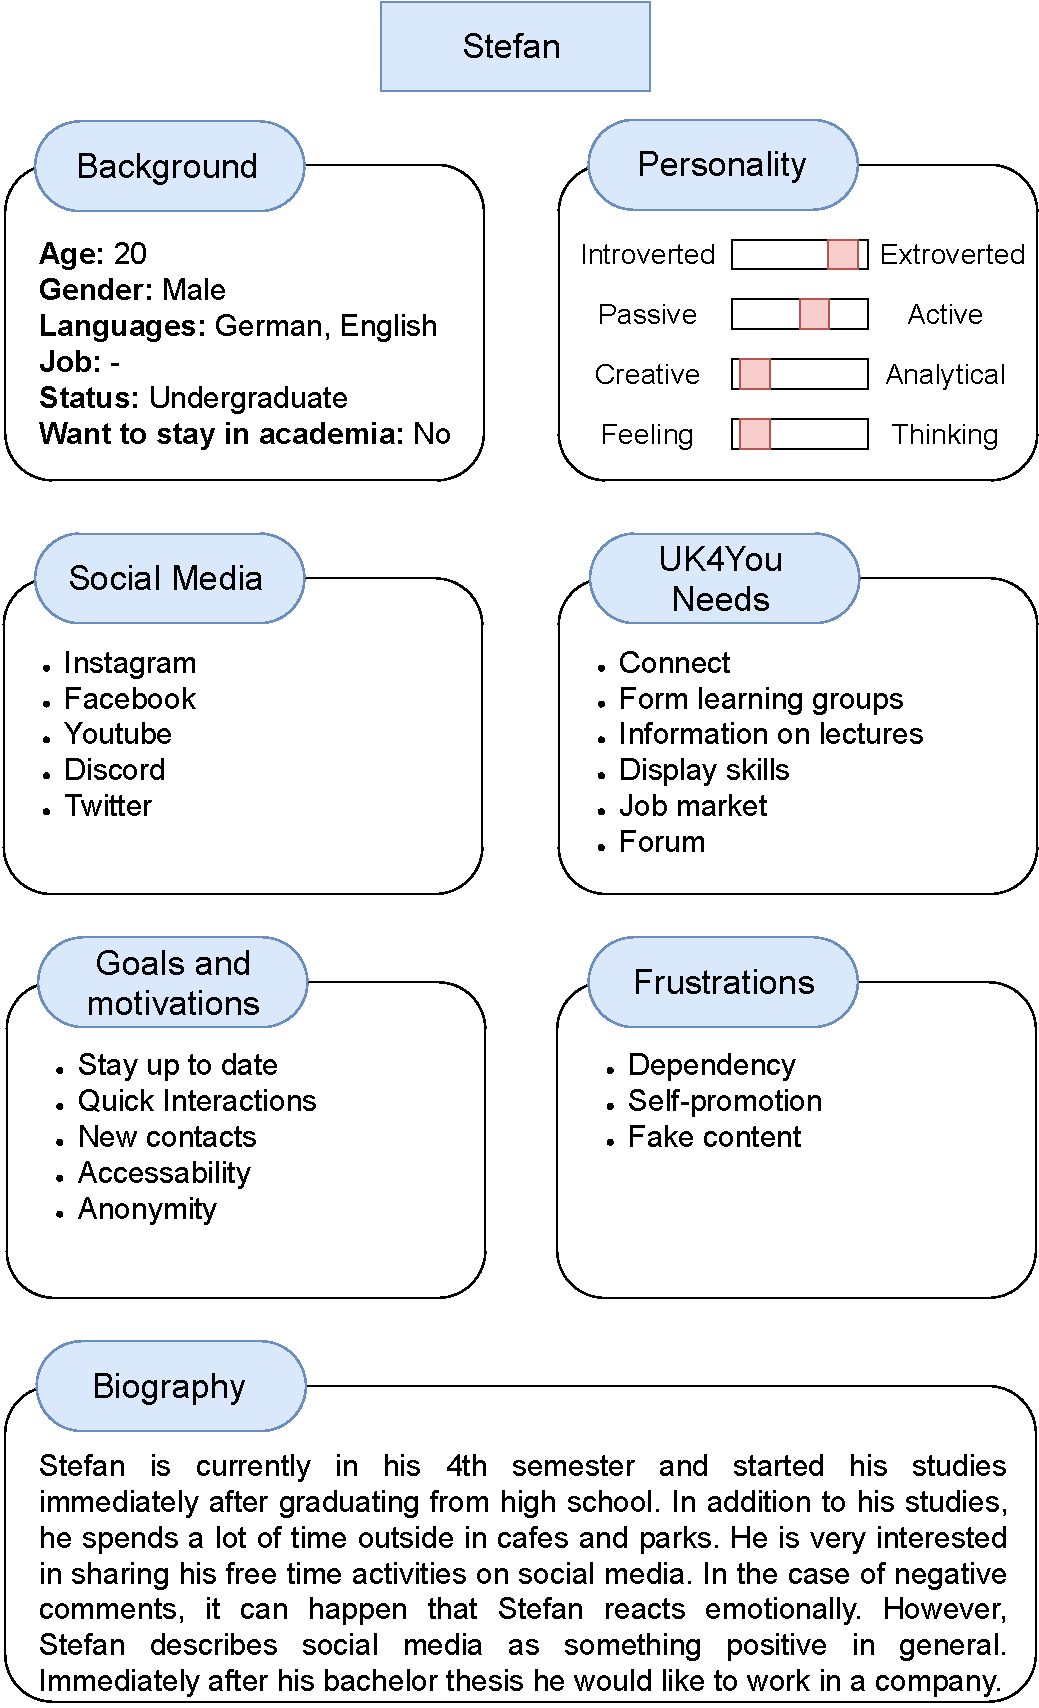
\includegraphics[width=0.8\columnwidth]{figures/Persona1.pdf}
    \caption{\label{fig:persona-one} Persona - Stefan}
\end{figure}

\begin{figure}[ht]
    \centering
    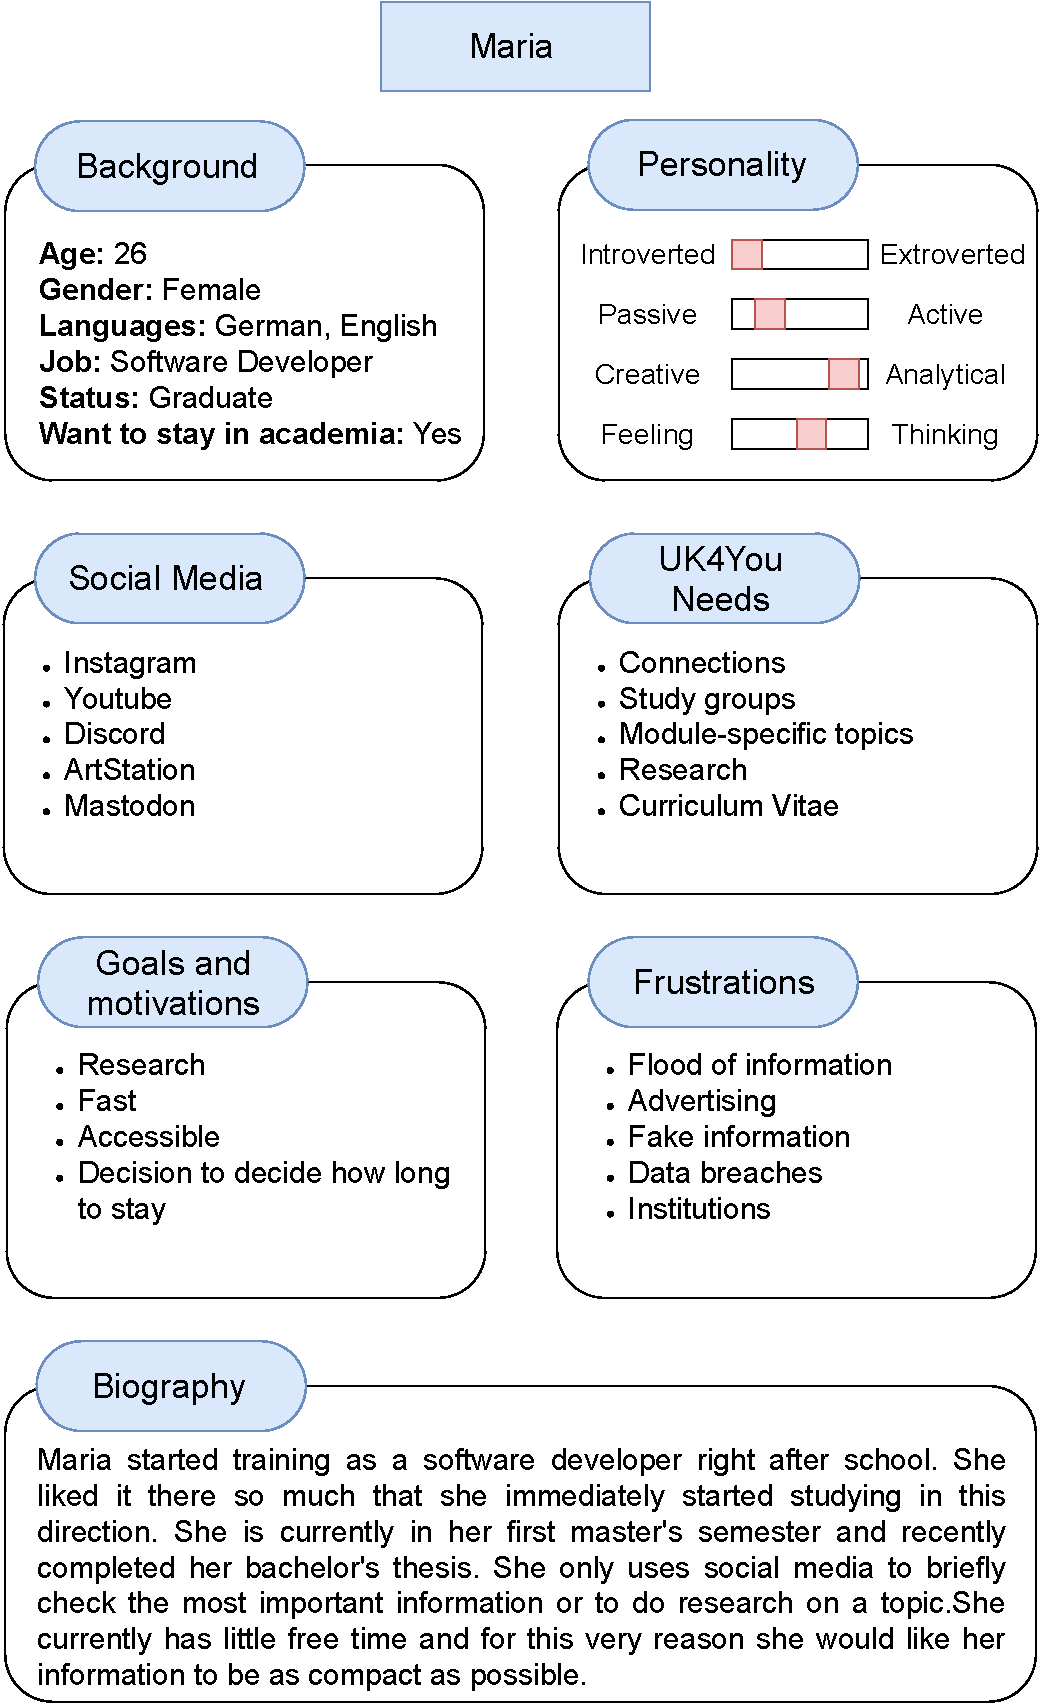
\includegraphics[width=0.8\columnwidth]{figures/Persona2.pdf}
    \caption{\label{fig:persona-two} Persona - Maria}
\end{figure}

\end{document}
